\chapter{Стереометрия: расстояния, сечения и сферы}\label{chap:exam-solid}\markright{Глава 32}

\section{Взаимное расположение прямых и плоскостей}
Формулы расстояния от точки до плоскости, углов, векторного произведения и объёмов введены в главе \ref{chap:solid-geometry}. Здесь они работают вместе с признаками параллельности и перпендикулярности. Плоскости обозначаются \(\alpha,\beta\); обозначение \((ABC)\) допустимо, только если \(A,B,C\) не лежат на одной прямой. Для куба \(ABCDA_1B_1C_1D_1\) верхние вершины находятся над соответствующими нижними.

\par\addvspace{2pt}\begin{lrbox}{\CatFlowBox}\begin{minipage}[t]{\linewidth}
\setlength{\parskip}{2pt}\setlength{\columnsep}{4.5mm}\setlength{\intextsep}{0pt}
\begin{wrapfigure}[9]{r}{54mm}

\includegraphics[width=54mm,height=58mm,keepaspectratio]{images/unique/art-248.png}
\end{wrapfigure}
Пространственный чертёж показывает расположение граней, но обычно не сохраняет ни длины, ни углы. На изображении куба квадратная грань выглядит параллелограммом, а перпендикулярные рёбра могут образовывать острый угол. Поэтому сначала полезно выбрать настоящую плоскость, внутри которой будет решаться часть задачи. Такой плоскостью может оказаться грань, диагональное сечение или плоскость через высоту пирамиды. В ней уже можно применять привычные теоремы о треугольниках. Если одна линия расположена вне выбранной плоскости, нельзя незаметно использовать её как сторону плоского угла. Сначала строят проекцию или проводят параллельную линию через подходящую точку. Эти небольшие проверки часто важнее длинного вычисления и предупреждают ошибку, которую трудно заметить по готовому рисунку.
\par\WFclear\end{minipage}\end{lrbox}%
\ifdim\dimexpr\ht\CatFlowBox+\dp\CatFlowBox\relax<58mm\dp\CatFlowBox=\dimexpr58mm-\ht\CatFlowBox\relax\fi%
\noindent\usebox{\CatFlowBox}\par\addvspace{2pt}
\begin{definition}\term{Прямая, параллельная плоскости} (\emph{line parallel to a plane}), не имеет с ней общих точек.
\par\term{Параллельные плоскости} (\emph{parallel planes}) — различные плоскости без общих точек.
\par\term{След секущей плоскости на грани} (\emph{trace on a face}) — её пересечение с плоскостью этой грани, если оно является прямой.\end{definition}
Прямая относительно плоскости либо содержится в ней, либо пересекает её в одной точке, либо параллельна ей. Две различные плоскости либо параллельны, либо пересекаются по прямой. Две прямые в пространстве могут также скрещиваться, как определено в главе \ref{chap:solid-geometry}.
\begin{theorem}[Признаки параллельности]\label{thm:exam-solid-parallel}
Если прямая не лежит в плоскости и параллельна некоторой прямой этой плоскости, она параллельна плоскости. Если две пересекающиеся прямые одной плоскости соответственно параллельны двум пересекающимся прямым другой, различные плоскости параллельны. При пересечении двух параллельных плоскостей третьей полученные прямые параллельны, если обе существуют.
\end{theorem}
\begin{proof}Направление первой прямой принадлежит двумерному пространству направлений плоскости. Поэтому при наличии общей точки вся прямая лежала бы в плоскости; это исключено условием. Во втором случае два независимых параллельных направления порождают одинаковые пространства направлений. Плоскости с такими направлениями при наличии общей точки совпадают, а иначе параллельны. Прямые последнего утверждения лежат в одной секущей плоскости; если бы пересекались, точка пересечения принадлежала бы обеим исходным параллельным плоскостям.\end{proof}
Условие «не лежит» в первом признаке обязательно. Параллельность двух выбранных рёбер также не доказывает параллельности содержащих их плоскостей: нужен второй независимый набор направлений.
\begin{example}\textbf{Разбор 1: доказать положение до вычислений.} В кубе прямая \(AB\) параллельна \(A_1B_1\), лежащей в верхней грани, и не лежит в этой грани. Поэтому \(AB\parallel(A_1B_1C_1)\). Верхняя и нижняя грани параллельны по двум парам пересекающихся рёбер. Однако плоскости \((ABB_1)\), \((DCC_1)\) нельзя объявлять перпендикулярными из-за вида рисунка: это противоположные, а значит, параллельные грани.\end{example}

\section{Проекции, три перпендикуляра и двугранный угол}
\begin{definition}\term{Ортогональная проекция точки} (\emph{orthogonal projection}) на плоскость — основание перпендикуляра к ней; точка самой плоскости проектируется в себя.
\par\term{Проекция отрезка} (\emph{segment projection}) соединяет проекции его концов.
\par\term{Наклонная} (\emph{oblique segment}) из точки вне плоскости соединяет её с точкой плоскости и не является перпендикуляром.\end{definition}
\begin{theorem}[Теорема о трёх перпендикулярах]\label{thm:exam-solid-three-perpendiculars}
Пусть \(AH\perp\alpha\), \(B\in\alpha\), \(B\ne H\), а прямая \(\ell\subset\alpha\) проходит через \(B\). Тогда \(\ell\perp AB\) равносильно \(\ell\perp HB\).
\end{theorem}
\par\addvspace{2pt}\begin{lrbox}{\CatFlowBox}\begin{minipage}[t]{\linewidth}
\setlength{\parskip}{2pt}\setlength{\columnsep}{4.5mm}\setlength{\intextsep}{0pt}
\begin{wrapfigure}[11]{l}{54mm}

\includegraphics[width=54mm,height=58mm,keepaspectratio]{images/unique/art-259.png}
\end{wrapfigure}
\textit{Доказательство.} Для направляющего вектора \(v\) прямой \(\ell\) имеем \(v\cdot\overrightarrow{HA}=0\). Поскольку \(\overrightarrow{BA}=\overrightarrow{BH}+\overrightarrow{HA}\), получаем \(v\cdot\overrightarrow{BA}=v\cdot\overrightarrow{BH}\). Одно скалярное произведение равно нулю ровно тогда, когда равно нулю другое. Прямые пересекаются в \(B\), поэтому это именно перпендикулярность прямых, а не только направлений.\hfill\(\blacksquare\)
\par\WFclear\end{minipage}\end{lrbox}%
\ifdim\dimexpr\ht\CatFlowBox+\dp\CatFlowBox\relax<58mm\dp\CatFlowBox=\dimexpr58mm-\ht\CatFlowBox\relax\fi%
\noindent\usebox{\CatFlowBox}\par\addvspace{2pt}

\begin{definition}\term{Двугранный угол} (\emph{dihedral angle}) образован двумя полуплоскостями с общей граничной прямой, называемой ребром.
\par\term{Линейный угол двугранного угла} (\emph{linear angle of a dihedral angle}) получают, выбирая на ребре точку и проводя в каждой из двух полуплоскостей луч, перпендикулярный ребру. Выбранные лучи лежат в одной плоскости, перпендикулярной ребру, и образуют угол от \(0^\circ\) до \(180^\circ\).\end{definition}
\begin{theorem}[Как найти двугранный угол]
Величина линейного угла не зависит от точки на ребре. Плоскость, содержащая прямую, перпендикулярную другой плоскости, перпендикулярна ей. Меньший угол между плоскостями с нормалями \(n_1,n_2\) удовлетворяет
\[
\cos\theta=\frac{|n_1\cdot n_2|}{\|n_1\|\|n_2\|}.
\]
Для конкретного двугранного угла нужно дополнительно выбрать полуплоскости: его величина может быть \(180^\circ-\theta\).
\end{theorem}
\begin{proof}При переносе вдоль ребра перпендикулярные ему лучи в тех же полуплоскостях переходят в параллельные сонаправленные лучи, а угол сохраняется. В сечении плоскостью, перпендикулярной ребру, нормали к исходным плоскостям перпендикулярны их следам. Углы между следами и нормалями равны либо дополнительны; модуль косинуса выбирает меньший. Если одна плоскость содержит нормаль к другой, в таком сечении один след перпендикулярен другому; линейный угол прямой.\end{proof}
\begin{example}\textbf{Разбор 2: грань правильной пирамиды.} Основание — квадрат со стороной \(10\), высота \(SO=12\), \(M\) — середина стороны основания. В основании \(OM=5\) и \(OM\) перпендикулярен этой стороне. По трём перпендикулярам \(SM\) тоже ей перпендикулярен. Поэтому линейный угол между боковой гранью и основанием равен \(\angle SMO\), а \(\operatorname{tg}\angle SMO=\frac{12}{5}\). Из прямоугольного \(SOM\) апофема \(SM=13\). Угол не заменяется углом между случайно выбранным боковым ребром и основанием.\end{example}
Для проекции отрезка длины \(L\), составляющего с плоскостью угол \(\alpha\), получаем \(L_{\mathrm{пр}}=L\cos\alpha\) из прямоугольного треугольника. При перпендикулярном положении проекция — точка. Площадь ортогональной проекции плоского многоугольника равна \(S|\cos\theta|\), где \(\theta\) — угол его плоскости с плоскостью проекции: разбиение на треугольники сводит доказательство к неизменной длине основания, параллельного линии пересечения плоскостей, и умножению соответствующей высоты на \(|\cos\theta|\). Для параллельных плоскостей площадь сохраняется, для перпендикулярных равна нулю.

\section{Расстояние как общий перпендикуляр}
\begin{definition}\term{Расстояние между множествами} (\emph{distance between sets}) — инфимум расстояний между их точками.
\par\term{Общий перпендикуляр скрещивающихся прямых} (\emph{common perpendicular}) — соединяющий точки этих прямых отрезок, перпендикулярный обеим.\end{definition}
\begin{theorem}[Расстояния между прямыми и плоскостями]\label{thm:exam-solid-distances}
Расстояние между параллельными плоскостями \(n\cdot x=d_1,n\cdot x=d_2\) равно \(\frac{|d_2-d_1|}{\|n\|}\). Для прямой, параллельной плоскости, подходит расстояние от любой её точки до плоскости. Для прямых \(a:A+tu\), \(b:B+sv\) с ненулевыми направлениями \(u,v\):
\[
d(a,b)=\frac{\|(B-A)\times u\|}{\|u\|}\quad(u\parallel v),
\qquad
d(a,b)=\frac{|(B-A)\cdot(u\times v)|}{\|u\times v\|}\quad(u\not\parallel v).
\]
Во втором случае нулевое расстояние означает пересечение, положительное — скрещивание.
\end{theorem}
\begin{proof}В первых двух утверждениях нормальная составляющая разности точек постоянна; перпендикуляр достигает её длины, как в формуле расстояния до плоскости. Для параллельных прямых удаление составляющей \(B-A\) вдоль \(u\) оставляет перпендикуляр длины \(\frac{\|(B-A)\times u\|}{\|u\|}\). Для непараллельных направлений \(n=u\times v\) перпендикулярен обоим. Нормальная составляющая любого соединяющего вектора равна \(\frac{(B-A)\cdot n}{\|n\|}\), поэтому это нижняя граница расстояния. Можно выбрать \(s,t\), чтобы соединяющий вектор был перпендикулярен \(u,v\): система двух линейных уравнений имеет определитель, по модулю равный \(\|u\times v\|^2>0\). Нижняя граница достигается на общем перпендикуляре. Если его длина нулевая, точки совпадают.\end{proof}
Эти формулы относятся к целым прямым. Для двух отрезков основания общего перпендикуляра могут оказаться вне отрезков; тогда минимальное расстояние дополнительно проверяют на их концах.
\begin{example}\textbf{Разбор 3: скрещивающиеся прямые.} Пусть \(a=(t,t,0)\), \(b=(1,s,s)\). Их направления \(u=(1,1,0)\), \(v=(0,1,1)\) имеют \(u\times v=(1,-1,1)\). Поэтому \(d=\frac{1}{\sqrt{3}}\). Проверим достижение: при \(t=\frac{2}{3},s=\frac{1}{3}\) соединяющий вектор равен \((\frac{1}{3},-\frac{1}{3},\frac{1}{3})\); его скалярные произведения с \(u,v\) равны нулю, а длина \(\frac{1}{\sqrt{3}}\). Прямые не пересекаются, потому что расстояние положительно.\end{example}

\section{Сечения: от трёх точек к многоугольнику}
\par\addvspace{2pt}\begin{lrbox}{\CatFlowBox}\begin{minipage}[t]{\linewidth}
\setlength{\parskip}{2pt}\setlength{\columnsep}{4.5mm}\setlength{\intextsep}{0pt}
\begin{wrapfigure}[11]{l}{54mm}

\includegraphics[width=54mm,height=58mm,keepaspectratio]{images/unique/art-249.png}
\end{wrapfigure}
При построении сечения каждую новую точку полезно связывать с конкретным ребром, а каждый новый отрезок с конкретной гранью. Точки на одной грани можно соединять сразу, если обе принадлежат секущей плоскости. Для точек на разных гранях такого разрешения пока нет: соединяющая их линия может пройти через внутренность тела и не быть стороной сечения. Удобно подписывать найденные вершины в порядке обхода, проверяя после каждого шага, на какой грани лежит очередная сторона. В конце контур должен замкнуться. Если появляется лишняя вершина или пересекаются несоседние стороны, стоит вернуться к последнему выбору грани. Координаты помогают проверить построение, но не заменяют объяснение того, какие части пересечения действительно принадлежат ограниченному многограннику.
\par\WFclear\end{minipage}\end{lrbox}%
\ifdim\dimexpr\ht\CatFlowBox+\dp\CatFlowBox\relax<58mm\dp\CatFlowBox=\dimexpr58mm-\ht\CatFlowBox\relax\fi%
\noindent\usebox{\CatFlowBox}\par\addvspace{2pt}
\begin{definition}\term{Сечение многогранника} (\emph{plane section of a polyhedron}) — его пересечение с плоскостью. Для выпуклого многогранника невырожденное сечение является выпуклым многоугольником; его стороны лежат на гранях, вершины — на рёбрах, кроме случаев прохождения плоскости через целое ребро.\end{definition}
\begin{theorem}[Проверка построения сечения]
Плоскость однозначно задаётся тремя неколлинеарными точками. Чтобы построить сечение выпуклого многогранника, достаточно найти пересечения этой плоскости со всеми рёбрами, оставить точки на отрезках рёбер и соединить их по общим граням. Следы на параллельных гранях параллельны. Для плоскости \(n\cdot x=d\) на ребре \(P+t(Q-P)\) точка пересечения определяется равенством
\[
t=\frac{d-n\cdot P}{n\cdot(Q-P)}.
\]
При ненулевом знаменателе она принадлежит ребру ровно при \(0\le t\le1\). Если знаменатель нулевой, ребро либо лежит в плоскости целиком, либо не пересекает её.
\end{theorem}
\begin{proof}Пересечение двух выпуклых множеств выпукло. Каждая сторона сечения находится в плоскости грани, а её концы достигаются на границе этой грани, то есть на рёбрах. Поэтому перечисление всех допустимых пересечений не теряет вершин. Параллельность следов следует из признака выше. Подстановка параметрического уравнения ребра даёт формулу и все исключительные случаи.\end{proof}
\begin{example}\textbf{Разбор 4: шесть шагов на кубе.} В кубе ребра \(a\) положим \(A=(0,0,0),B=(a,0,0),C=(a,a,0),D=(0,a,0)\), верхние вершины имеют \(z=a\). Плоскость проходит через середины \(BC,CD,DD_1\).
\begin{enumerate}
\item Координаты данных точек \((a,\frac{a}{2},0),(\frac{a}{2},a,0),(0,a,\frac{a}{2})\) дают уравнение \(x+y+z=\frac{3a}{2}\).
\item На нижней грани получаем сторону между первыми двумя точками.
\item На грани \(y=a\) соединяем вторую и третью.
\item На грани \(x=0\) следующая вершина \((0,\frac{a}{2},a)\); на верхней грани следующая \((\frac{a}{2},0,a)\).
\item На грани \(y=0\) получаем \((a,0,\frac{a}{2})\); последняя сторона лежит на \(x=a\) и возвращает нас к первой точке.
\item Остальные рёбра не дают новых пересечений при \(0\le t\le1\).
\end{enumerate}
Все шесть сторон имеют длину \(\frac{a}{\sqrt{2}}\), а скалярные произведения соседних направлений дают внутренние углы \(120^\circ\). Сечение — правильный шестиугольник площади \(\frac{3\sqrt3\,a^2}{4}\).\end{example}
\begin{example}\textbf{Разбор 5: сечение пирамиды и две проверки.} В пирамиде \(SABCD\) точки \(M,N,P\) — середины \(SA,SB,SC\). В гранях \(SAB,SBC\) средние линии \(MN,NP\) параллельны \(AB,BC\); значит, \((MNP)\parallel(ABC)\). В грани \(SAD\) проводим из \(M\) параллель к \(AD\); она пересекает \(SD\) в его середине \(Q\). Стороны сечения последовательно лежат на \(SAB,SBC,SCD,SDA\), контур \(MNPQ\) замкнут. По подобию его площадь равна четверти площади основания; объём верхней пирамиды — одной восьмой полного объёма. Нижняя усечённая часть имеет оставшиеся семь восьмых. Уравнение плоскости здесь не требовалось.\end{example}
\begin{center}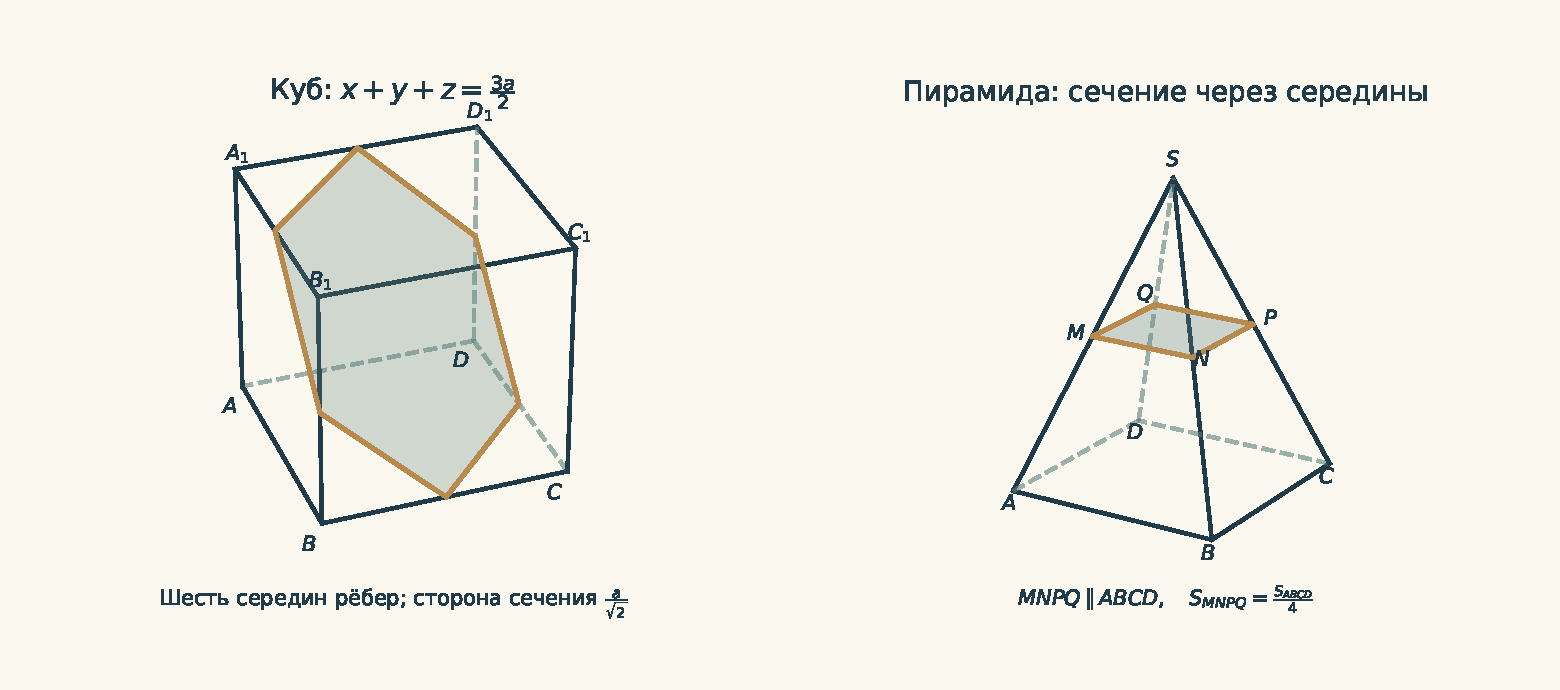
\includegraphics[width=\linewidth]{images/exam-geometry-sections.pdf}\end{center}


\section{Правильные призмы, пирамиды и усечённые тела}
\par\addvspace{2pt}\begin{lrbox}{\CatFlowBox}\begin{minipage}[t]{\linewidth}
\setlength{\parskip}{2pt}\setlength{\columnsep}{4.5mm}\setlength{\intextsep}{0pt}
\begin{wrapfigure}[11]{r}{54mm}
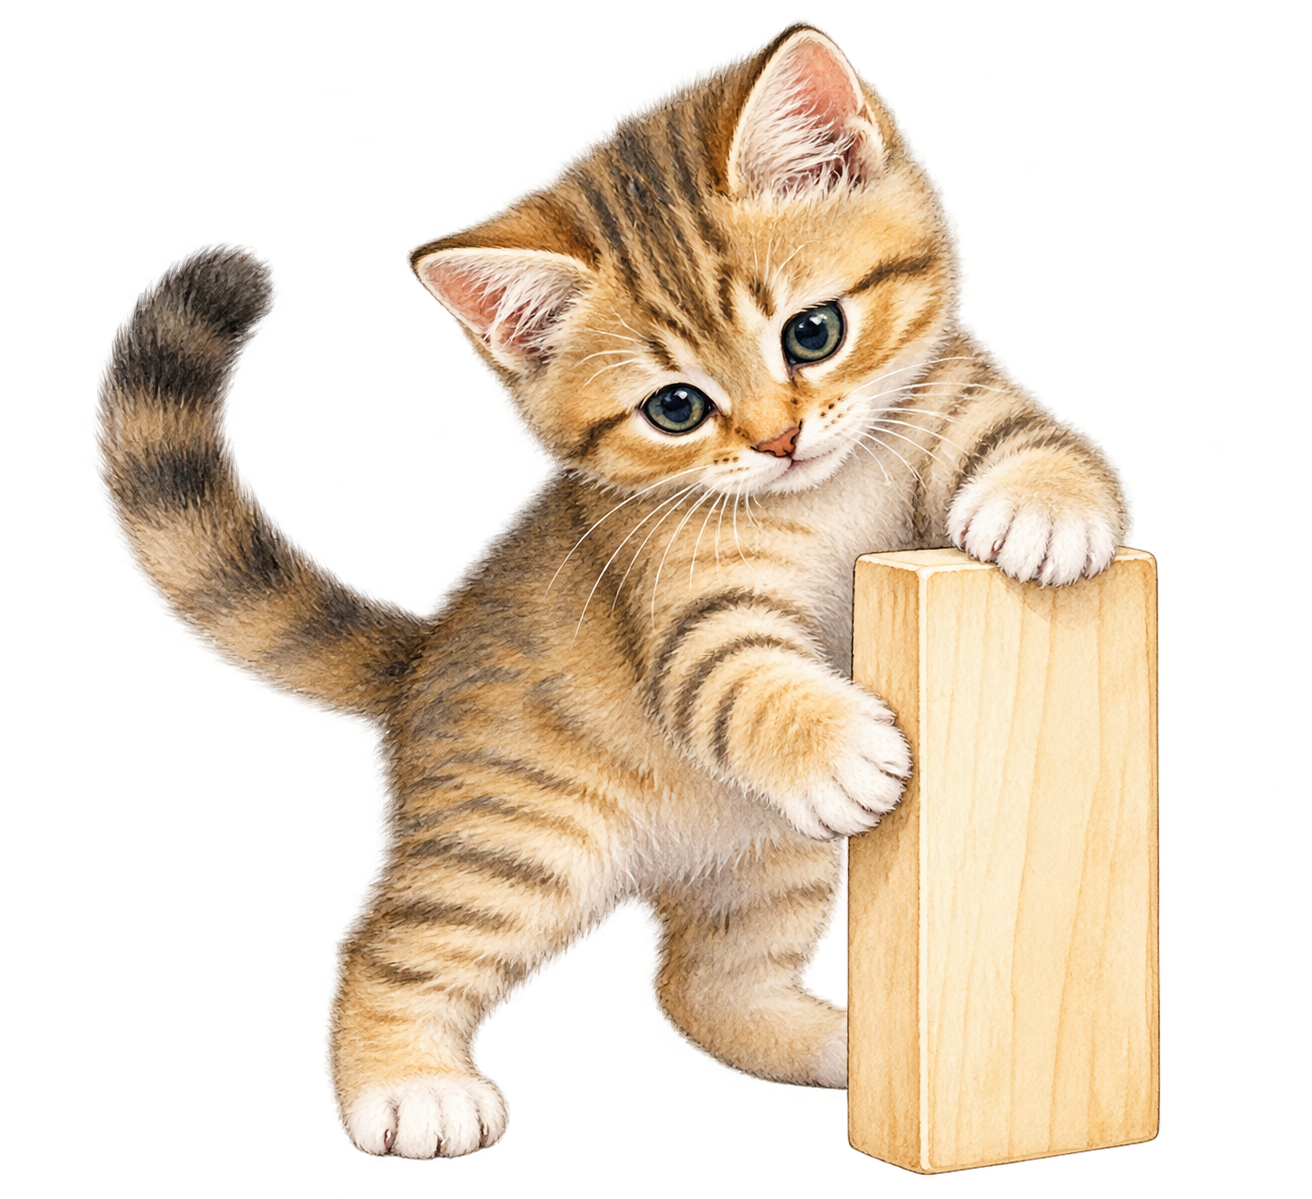
\includegraphics[width=54mm,height=58mm,keepaspectratio]{images/unique/art-250.png}
\end{wrapfigure}
Формула площади поверхности требует понимать, какие именно грани входят в ответ. Если тело закрыто, к боковой поверхности добавляют оба основания призмы или основание пирамиды. Если речь идёт о развёртке, одинаковые рёбра на рисунке могут изображаться несколько раз, но площадь каждой грани учитывают только один раз. В правильной пирамиде важно различать высоту тела, высоту боковой грани и боковое ребро. Эти три отрезка обычно имеют разные длины и участвуют в разных прямоугольных треугольниках. Перед подстановкой чисел удобно обозначить центр основания, середину его стороны и вершину. После этого каждая нужная длина получается из своего треугольника, а выбор формулы перестаёт зависеть от запоминания похожих букв.
\par\WFclear\end{minipage}\end{lrbox}%
\ifdim\dimexpr\ht\CatFlowBox+\dp\CatFlowBox\relax<58mm\dp\CatFlowBox=\dimexpr58mm-\ht\CatFlowBox\relax\fi%
\noindent\usebox{\CatFlowBox}\par\addvspace{2pt}
\begin{definition}\term{Правильная призма} (\emph{regular prism}) — прямая призма с правильным многоугольником в основании.
\par\term{Правильная пирамида} (\emph{regular pyramid}) имеет правильное основание, а основание её высоты совпадает с центром этого многоугольника.
\par\term{Апофема правильной пирамиды} (\emph{slant height}) — высота её боковой грани из вершины.
\par\term{Усечённая пирамида} (\emph{pyramidal frustum}) получается удалением от пирамиды верхней части плоскостью, параллельной основанию.
\par\term{Правильный многогранник} (\emph{regular polyhedron}) — выпуклый многогранник с равными правильными многоугольными гранями и одинаковым числом сходящихся в каждой вершине рёбер; куб и правильный тетраэдр — примеры.\end{definition}
\begin{theorem}[Поверхности и усечённая пирамида]\label{thm:exam-solid-areas}
У прямой призмы \(S_{\mathrm{бок}}=Ph\), \(S_{\mathrm{полн}}=Ph+2B\), где \(P,B\) — периметр и площадь основания. У правильной пирамиды с высотой \(h\), апофемой \(l\), радиусами основания \(r_b,R_b\):
\[
l=\sqrt{h^2+r_b^2},\quad e=\sqrt{h^2+R_b^2},\quad
S_{\mathrm{бок}}=\frac{1}{2}Pl,\quad S_{\mathrm{полн}}=B+\frac{1}{2}Pl.
\]
У правильной усечённой пирамиды с площадями оснований \(B_1,B_2\), периметрами \(P_1,P_2\), высотой \(h\) и апофемой \(l\):
\[
l=\sqrt{h^2+(r_1-r_2)^2},\quad
S_{\mathrm{бок}}=\frac{P_1+P_2}{2}l,\quad
V=\frac{h}{3}(B_1+B_2+\sqrt{B_1B_2}).
\]
Для полной поверхности добавляют оба основания.
\end{theorem}
\begin{proof}Боковые грани прямой призмы — прямоугольники высоты \(h\); складывание их площадей даёт \(Ph\). В правильной пирамиде треугольники от центра основания к его вершине или середине стороны прямоугольные; Пифагор даёт \(e,l\). Сложение площадей боковых треугольников даёт \(\frac{Pl}{2}\).
В осевом сечении усечённой пирамиды разность радиусов вписанных окружностей оснований и высота являются катетами для \(l\). Боковые грани — трапеции общей высоты \(l\); сумма их площадей даёт формулу. Для объёма пусть большие и малые линейные размеры оснований равны \(\lambda,\mu\), \(\lambda>\mu>0\); их площади \(c\lambda^2,c\mu^2\), высоты исходных подобных пирамид \(H\lambda,H\mu\). Разность объёмов равна \(\frac{cH(\lambda^3-\mu^3)}{3}\), а \(h=H(\lambda-\mu)\). Разложение разности кубов даёт формулу. Если верхнее основание вырождается в вершину, формула переходит в \(V=\frac{B_1h}{3}\).\end{proof}
\begin{example}\textbf{Разбор 6: усечённая квадратная пирамида.} Стороны нижнего и верхнего оснований равны \(8,4\), высота \(3\). Радиусы вписанных окружностей оснований \(4,2\), поэтому апофема \(\sqrt{3^2+(4-2)^2}=\sqrt{13}\). Периметры \(32,16\); боковая площадь \(24\sqrt{13}\), полная \(80+24\sqrt{13}\). Объём равен \(\frac{3}{3}(64+16+\sqrt{64\cdot16})=112\). Боковое ребро здесь не равно апофеме; подставлять его вместо высоты трапециевидной грани нельзя.\end{example}

\section{Сфера в теле и сфера около тела}
\begin{definition}\term{Вписанная сфера} (\emph{insphere}) многогранника ограничивает шар, лежащий внутри и касающийся всех его граней.
\par\term{Описанная сфера} (\emph{circumsphere}) проходит через все вершины многогранника. Её центр не обязан лежать внутри.
\par\term{Касательная плоскость к сфере} (\emph{tangent plane to a sphere}) имеет со сферой ровно одну общую точку.\end{definition}
\begin{theorem}[Сечение сферы и касательная плоскость]
Плоскость на расстоянии \(d<R\) от центра сферы радиуса \(R\) даёт окружность радиуса \(\sqrt{R^2-d^2}\). При \(d=R\) остаётся одна точка, а при \(d>R\) пересечения нет. Касательная плоскость перпендикулярна радиусу в точке касания.
\end{theorem}
\par\addvspace{2pt}\begin{lrbox}{\CatFlowBox}\begin{minipage}[t]{\linewidth}
\setlength{\parskip}{2pt}\setlength{\columnsep}{4.5mm}\setlength{\intextsep}{0pt}
\begin{wrapfigure}[12]{l}{54mm}

\includegraphics[width=54mm,height=58mm,keepaspectratio]{images/unique/art-251.png}
\end{wrapfigure}
\textit{Доказательство.} Проекция центра на плоскость является центром сечения; Пифагор даёт \(r^2+d^2=R^2\). При равенстве расстояния радиусу единственная точка — основание перпендикуляра; при большем расстоянии ни одна точка плоскости не достигает сферы. Это также доказывает характеристику касательной плоскости.\hfill\(\blacksquare\)
\par\WFclear\end{minipage}\end{lrbox}%
\ifdim\dimexpr\ht\CatFlowBox+\dp\CatFlowBox\relax<58mm\dp\CatFlowBox=\dimexpr58mm-\ht\CatFlowBox\relax\fi%
\noindent\usebox{\CatFlowBox}\par\addvspace{2pt}

\begin{theorem}[Радиусы для правильных тел]\label{thm:exam-solid-spheres}
Для прямой призмы с циклическим основанием радиуса \(R_b\) радиус описанной сферы
\[
R=\sqrt{R_b^2+\frac{h^2}{4}}.
\]
В правильную призму можно вписать сферу ровно при \(h=2r_b\); её радиус тогда \(r_b\). Для правильной пирамиды
\[
r=\frac{3V}{S_{\mathrm{полн}}}=\frac{r_bh}{l+r_b},\qquad
R=\frac{h^2+R_b^2}{2h}.
\]
Центр описанной сферы расположен на оси на направленной высоте \(z=\frac{h^2-R_b^2}{2h}\) от основания.
\end{theorem}
\begin{proof}Центр сферы призмы расположен над центром окружности основания посередине между основаниями. До каждой вершины расстояние \(\sqrt{R_b^2+\frac{h^2}{4}}\). Для вписанной сферы равные расстояния до оснований требуют средней высоты \(\frac{h}{2}\), а касания боковых граней правильной призмы требуют точки на оси и расстояния \(r_b\); отсюда необходимость и достаточность \(h=2r_b\).
В правильной пирамиде точка на оси высоты \(z\) находится на расстоянии \(z\) от основания и \(\frac{r_b(h-z)}{l}\) от каждой боковой грани. Равенство даёт \(z=\frac{r_bh}{l+r_b}\) между \(0,h\), а основания перпендикуляров принадлежат граням. Поэтому вписанная сфера существует. Соединение её центра со всеми гранями разбивает тело на пирамиды высоты \(r\), значит, \(V=\frac{rS_{\mathrm{полн}}}{3}\).
Для описанной сферы при осевом центре требуются равные квадраты расстояний до вершины и вершин основания: \((h-z)^2=R_b^2+z^2\). Решение даёт указанные \(z,R=h-z>0\). Если \(h<R_b\), центр ниже основания; это не мешает описанности.\end{proof}
Для цилиндра под описанной сферой понимаем сферу через обе окружности оснований, а для конуса — через вершину и окружность основания. Для цилиндра аналогичное осевое сечение даёт описанную сферу \(R=\sqrt{r_b^2+\frac{h^2}{4}}\), а вписанная возможна при \(h=2r_b\). Для прямого кругового конуса осевое сечение — равнобедренный треугольник, поэтому \(r=\frac{r_bh}{\sqrt{h^2+r_b^2}+r_b}\), \(R=\frac{h^2+r_b^2}{2h}\). Эти формулы также следуют из только что приведённых расстояний до основания и образующих.

\section{Координатный метод как проверка геометрии}
Для плоскости через точки \(P,Q,R\) вычисляют ненулевую нормаль \(n=(Q-P)\times(R-P)\), затем пишут \(n\cdot(x-P)=0\). Нулевая нормаль означает, что точки коллинеарны и единственная плоскость ими не определена. Угол между прямой направления \(u\) и плоскостью вычисляют через \(\sin\alpha=\frac{|u\cdot n|}{\|u\|\|n\|}\), а объём тетраэдра — как шестую часть модуля смешанного произведения трёх рёбер из одной вершины. Обоснования даны в главе \ref{chap:solid-geometry}.
Координаты выбирают после анализа условий: в кубе удобно направить оси по трём рёбрам, в правильной пирамиде — поместить основание в \(z=0\), ось высоты в \(Oz\). Тогда проверяются не впечатления от изображения, а точные скалярные произведения, уравнения и интервалы параметров.

\relax

\par\addvspace{2pt}\begin{lrbox}{\CatFlowBox}\begin{minipage}[t]{\linewidth}
\setlength{\parskip}{2pt}\setlength{\columnsep}{4.5mm}\setlength{\intextsep}{0pt}
\begin{wrapfigure}[13]{l}{54mm}

\includegraphics[width=54mm,height=58mm,keepaspectratio]{images/unique/art-271.png}
\end{wrapfigure}
Пространственное сечение определяется плоскостью, а нарисованный многоугольник должен целиком лежать в этой плоскости. Поэтому найденные точки на рёбрах проверяют на планарность, а затем устанавливают порядок его сторон. Площадь сечения зависит от угла и высоты; равенство длин на перспективном рисунке не является данными задачи. При сравнении тел важно различать подобие всего пространства и изменение только основания. Если высота призмы остаётся прежней, масштаб основания не даёт обычного кубического закона для объёма и квадратного закона для каждой площади. Угол между плоскостями также требует выбора соответствующих перпендикулярных направлений, а не произвольных видимых рёбер.
\par\WFclear\end{minipage}\end{lrbox}%
\ifdim\dimexpr\ht\CatFlowBox+\dp\CatFlowBox\relax<61mm\dp\CatFlowBox=\dimexpr61mm-\ht\CatFlowBox\relax\fi%
\noindent\usebox{\CatFlowBox}\par\addvspace{2pt}
\relax
\section{Сечение с неизвестной высотой тела}
\begin{example}[Равнобедренность без измерений по картинке]\label{ex:review-ege-exam-solid-1}
В правильной треугольной призме \(ABCA_1B_1C_1\) сторона основания \(4\), высота \(h>0\). Плоскость проходит через \(A_1,B\) и середину \(M\) ребра \(CC_1\). Введём координаты
\[
A=(0,0,0),\ B=(4,0,0),\ C=(2,2\sqrt3,0),\ A_1=(0,0,h).
\]
Тогда \(M=(2,2\sqrt3,\frac h2)\), середина \(A_1B\) — \(H=(2,0,\frac h2)\). Вектор \(HM=(0,2\sqrt3,0)\) перпендикулярен \(A_1B\), поэтому \(MH\) — высота и медиана треугольника \(A_1BM\), он равнобедренный.
Это действительно всё сечение. Его плоскость имеет уравнение \(z=h(1-\frac x4)\). В треугольном основании все точки удовлетворяют \(0\le x\le4\), так что \(0\le z\le h\); проекция сечения на основание — весь треугольник \(ABC\), вершины которого поднимаются в \(A_1,B,M\). Дополнительных вершин нет.
Если площадь сечения \(12\), то
\[
12=\frac12\sqrt{16+h^2}\cdot2\sqrt3,
\quad h^2=32,\quad h=4\sqrt2.
\]
Отрицательное значение высоты геометрически недопустимо.
\end{example}

\begin{example}[Ромб определяет положение секущей плоскости]\label{ex:review-ege-exam-solid-2}
В правильной квадратной призме сторона основания \(a\), высота \(h>0\). Сечение через противоположные вершины \(D\) нижнего и \(B_1\) верхнего основания пересекает \(AA_1,CC_1\) в \(M,K\). Положим \(A=(0,0,0),B=(a,0,0),D=(0,a,0)\), \(M=(0,0,m)\). Уравнение плоскости:
\[
z=m+\frac{h-m}{a}x-\frac ma y.
\]
В точке \(K\) получаем \(k=h-m\). Поэтому \(M+K=B_1+D\): диагонали четырёхугольника \(MB_1KD\) имеют общую середину, и это параллелограмм. Для ромба соседние стороны должны быть равны:
\[
a^2+(h-m)^2=a^2+m^2,
\quad m=\frac h2.
\]
Значит, обе точки делят боковые рёбра пополам. Диагонали ромба имеют длины \(a\sqrt2\), \(\sqrt{2a^2+h^2}\) и перпендикулярны; его площадь
\[
S=\frac{a\sqrt2}{2}\sqrt{2a^2+h^2}.
\]
При \(a=2,S=4\sqrt2\) получаем \(h=2\sqrt2\). Сначала условие ромба нашло положение плоскости, и лишь затем площадь нашла высоту.
\end{example}

\section{Меняется основание, но сохраняется высота}
\begin{theorem}[Боковая площадь меньшей призмы]
В треугольной призме возьмём треугольник основания, полученный гомотетией с центром в одной вершине и коэффициентом \(0<k<1\). Через его вершины проведём отрезки, равные и параллельные боковым рёбрам исходной призмы. Боковая площадь полученной призмы равна \(kS_{\rm бок}\), а её объём равен \(k^2V\).
\end{theorem}
\begin{proof}
Соответствующие стороны оснований параллельны и имеют отношение \(k\). Каждая боковая грань — параллелограмм: одна его сторона уменьшена в \(k\), другая, параллельная боковому ребру, сохранена, угол между ними тот же. Поэтому площадь каждой боковой грани умножена на \(k\); складывая, получаем первое равенство и для наклонной призмы. Площадь основания умножена на \(k^2\), расстояние между плоскостями оснований прежнее; формула объёма даёт второе равенство. Эти две призмы в целом не подобны, поскольку вертикальное направление не масштабировалось.
\end{proof}
При средней линии основания \(k=\frac12\): боковая площадь уменьшается вдвое, объём — вчетверо. Правила \(k^2\) для всей поверхности и \(k^3\) для объёма относятся к подобным телам, где изменены все линейные размеры.
\Needspace{7\baselineskip}\section*{Задачи}
\begingroup\setlength{\parskip}{1pt}
\noindent\begin{minipage}[t]{\linewidth}\textbf{32.1.}\starmark{} В кубе \(ABCDA_1B_1C_1D_1\) докажи параллельность плоскостей \((ABB_1)\) и \((DCC_1)\).\par\end{minipage}\par
\noindent\begin{minipage}[t]{\linewidth}\textbf{32.2.} Почему в признаке параллельности прямой и плоскости нельзя опустить условие, что прямая не лежит в плоскости? Приведи координатный пример.\par\end{minipage}\par
\noindent\begin{minipage}[t]{\linewidth}\textbf{32.3.} Достаточно ли одной пары параллельных прямых для параллельности двух плоскостей? Приведи контрпример.\par\end{minipage}\par
\noindent\begin{minipage}[t]{\linewidth}\textbf{32.4.}\starmark{} Даны \(A=(0,0,5),H=(0,0,0),B=(3,4,0)\). Прямая \(\ell\) проходит через \(B\) с направлением \((-4,3,0)\). Докажи \(\ell\perp AB\), используя проекцию.\par\end{minipage}\par
\noindent\begin{minipage}[t]{\linewidth}\textbf{32.5.} Наклонная длины \(13\) соединяет точку с плоскостью. Косинус её угла с плоскостью равен \(\dfrac{12}{13}\). Найди длину проекции и расстояние от точки до плоскости.\par\end{minipage}\par
\par\addvspace{2pt}\begin{lrbox}{\CatFlowBox}\begin{minipage}[t]{\linewidth}
\setlength{\parskip}{2pt}\setlength{\columnsep}{4.5mm}\setlength{\intextsep}{0pt}
\begin{wrapfigure}[9]{r}{54mm}

\includegraphics[width=54mm,height=58mm,keepaspectratio]{images/unique/art-252.png}
\end{wrapfigure}
\textbf{32.6.} У правильной квадратной пирамиды сторона основания \(6\), высота \(4\). Найди апофему и тангенс двугранного угла при основании.\par

\textbf{32.7.} Плоская фигура площади \(24\) проектируется ортогонально на плоскость под углом \(60^\circ\) к её собственной плоскости. Найди площадь проекции.\par

\textbf{32.8.} Прямая \(a=(t,-t,2)\) и плоскость \(x+y+z=5\). Докажи параллельность и найди расстояние.\par

\textbf{32.9.} Найди расстояние между плоскостями \(2x-y+2z=1\) и \(2x-y+2z=10\).\par
\par\WFclear\end{minipage}\end{lrbox}%
\ifdim\dimexpr\ht\CatFlowBox+\dp\CatFlowBox\relax<58mm\dp\CatFlowBox=\dimexpr58mm-\ht\CatFlowBox\relax\fi%
\noindent\usebox{\CatFlowBox}\par\addvspace{2pt}

\noindent\begin{minipage}[t]{\linewidth}\textbf{32.10.} Найди расстояние от \(P=(1,2,3)\) до оси \(z\) и укажи ближайшую точку.\par\end{minipage}\par
\noindent\begin{minipage}[t]{\linewidth}\textbf{32.11.} Параллельные прямые заданы \((t,0,0)\) и \((s,3,4)\). Найди расстояние и один общий перпендикуляр.\par\end{minipage}\par
\noindent\begin{minipage}[t]{\linewidth}\textbf{32.12.} В кубе ребра \(a>0\) найди расстояние между прямыми \(AB\) и \(CC_1\). Обоснуй, что это скрещивающиеся прямые.\par\end{minipage}\par
\noindent\begin{minipage}[t]{\linewidth}\textbf{32.13.} Для прямых \((t,t,0)\) и \((1,s,s)\) найди расстояние через смешанное произведение.\par\end{minipage}\par
\noindent\begin{minipage}[t]{\linewidth}\textbf{32.14.} Найди концы общего перпендикуляра к прямым \((t,0,0)\) и \((0,2+s,3)\).\par\end{minipage}\par
\noindent\begin{minipage}[t]{\linewidth}\textbf{32.15.} Опиши линию пересечения плоскостей \(x+y+z=1\), \(x-y=0\).\par\end{minipage}\par
\noindent\begin{minipage}[t]{\linewidth}\textbf{32.16.} Куб ребра \(2\) пересечён плоскостью через середины \(BC,CD,DD_1\). Назови вид сечения, найди сторону и площадь.\par\end{minipage}\par
\noindent\begin{minipage}[t]{\linewidth}\textbf{32.17.} В кубе \([0,a]^3\) построй сечение \(x+y+z=a\). Найди площадь и объём части, содержащей начало координат.\par\end{minipage}\par
\noindent\begin{minipage}[t]{\linewidth}\textbf{32.18.}\starmark{} В пирамиде \(SABCD\) построй сечение через середины \(SA,SB,SC\) и найди отношение объёма верхней части к объёму всей пирамиды.\par\end{minipage}\par
\noindent\begin{minipage}[t]{\linewidth}\textbf{32.19.}\starmark{} Объясни на примере куба, почему соединение двух вершин сечения не всегда является его стороной. Возьми сечение \(ACC_1A_1\).\par\end{minipage}\par
\noindent\begin{minipage}[t]{\linewidth}\textbf{32.20.} Проверь пересечение ребра \(P=(0,0,0),Q=(1,1,1)\) с плоскостями \(x+y+z=2\) и \(x+y+z=4\).\par\end{minipage}\par
\noindent\begin{minipage}[t]{\linewidth}\textbf{32.21.} У правильной треугольной призмы сторона основания \(6\), высота \(8\). Найди боковую и полную площади поверхности и объём.\par\end{minipage}\par
\noindent\begin{minipage}[t]{\linewidth}\textbf{32.22.}\starmark{} Нижнее основание наклонной призмы — единичный квадрат в \(z=0\), верхнее получается переносом на \((1,0,1)\). Докажи, что формула \(S_{\mathrm{бок}}=P e\), где \(e\) — боковое ребро, здесь неверна.\par\end{minipage}\par
\noindent\begin{minipage}[t]{\linewidth}\textbf{32.23.} У правильной квадратной пирамиды сторона основания \(6\), высота \(4\). Найди боковое ребро, полную площадь и объём.\par\end{minipage}\par
\noindent\begin{minipage}[t]{\linewidth}\textbf{32.24.} У правильной усечённой квадратной пирамиды стороны оснований \(10,4\), высота \(4\). Найди апофему, полную площадь и объём.\par\end{minipage}\par
\noindent\begin{minipage}[t]{\linewidth}\textbf{32.25.} Площади оснований усечённой пирамиды равны \(9,4\), высота \(6\). Найди объём.\par\end{minipage}\par
\noindent\begin{minipage}[t]{\linewidth}\textbf{32.26.} Основание прямой призмы вписано в окружность радиуса \(5\), высота призмы \(24\). Найди радиус описанной сферы и положение центра.\par\end{minipage}\par
\noindent\begin{minipage}[t]{\linewidth}\textbf{32.27.} У правильной шестиугольной призмы сторона основания \(2\). При какой высоте существует вписанная сфера? Найди её радиус и радиус описанной сферы при этой высоте.\par\end{minipage}\par
\noindent\begin{minipage}[t]{\linewidth}\textbf{32.28.} У правильной квадратной пирамиды сторона основания \(6\), высота \(4\). Найди радиусы вписанной и описанной сфер. Где находится центр описанной?\par\end{minipage}\par
\noindent\begin{minipage}[t]{\linewidth}\textbf{32.29.} Сфера радиуса \(5\) пересечена плоскостью на расстоянии \(3\) от центра. Найди радиус окружности сечения и площадь соответствующего круга.\par\end{minipage}\par
\noindent\begin{minipage}[t]{\linewidth}\textbf{32.30.} Центр сферы \(O=(1,-1,2)\), радиус \(3\). Исследуй плоскости \(x=4\) и \(z=6\); укажи точку касания, если она есть.\par\end{minipage}\par
\noindent\begin{minipage}[t]{\linewidth}\textbf{32.31.} У цилиндра радиус основания \(2\), высота \(4\). Найди радиусы вписанной и описанной сфер.\par\end{minipage}\par
\noindent\begin{minipage}[t]{\linewidth}\textbf{32.32.} У прямого кругового конуса радиус основания \(3\), высота \(4\). Найди радиусы вписанной и описанной сфер.\par\end{minipage}\par
\noindent\begin{minipage}[t]{\linewidth}\textbf{32.33.} У правильного тетраэдра ребро \(2\sqrt6\). Найди радиусы вписанной и описанной сфер.\par\end{minipage}\par
\noindent\begin{minipage}[t]{\linewidth}\textbf{32.34.} В кубе найди угол пространственной диагонали \(AC_1\) с основанием и меньший угол плоскостей \((AB_1D_1)\), \((ABC)\).\par\end{minipage}\par
\noindent\begin{minipage}[t]{\linewidth}\textbf{32.35.} Плоскость проходит через \(A=(1,0,0),B=(0,2,0),C=(0,0,3)\). Найди её уравнение, расстояние от начала координат и объём тетраэдра \(OABC\).\par\end{minipage}\par
\noindent\begin{minipage}[t]{\linewidth}\textbf{32.36.}\starmark{} Можно ли единственным образом задать плоскость точками \((0,0,0),(1,1,1),(2,2,2)\)? Объясни нулевое векторное произведение и приведи две подходящие плоскости.\par\end{minipage}\par
\noindent\begin{minipage}[t]{\linewidth}\textbf{32.37.}\starmark{} В правильном тетраэдре \(ABCD\) точки \(M,K\) — середины \(AB,AD\). Найди отношение объёмов двух частей, на которые плоскость \(CMK\) делит тетраэдр, и косинус угла между \(AC\) и этой плоскостью.\par\end{minipage}\par
\noindent\begin{minipage}[t]{\linewidth}\textbf{32.38.} Цилиндр описан около шара и имеет объём \(30\). Найди объём шара, не вычисляя радиус.\par\end{minipage}\par
\noindent\begin{minipage}[t]{\linewidth}\textbf{32.39.}\starmark{} У правильной треугольной призмы сторона основания \(6\). Плоскость проходит через \(A_1,B\) и середину \(M\) ребра \(CC_1\). Докажи, что сечение — равнобедренный треугольник, и найди высоту призмы, если площадь сечения равна \(18\).\par\end{minipage}\par
\noindent\begin{minipage}[t]{\linewidth}\textbf{32.40.}\starmark{} Площадь основания правильной квадратной призмы \(9\). Сечение \(MB_1KD\), где \(M\in AA_1,K\in CC_1\), является ромбом площади \(15\). Докажи, что \(M,K\) — середины рёбер, и найди высоту.\par\end{minipage}\par
\noindent\begin{minipage}[t]{\linewidth}\textbf{32.41.} В основании треугольной призмы выделили подобный треугольник с коэффициентом \(\dfrac23\), стороны которого параллельны сторонам основания. Над ним построили призму с теми же боковыми рёбрами. У исходной призмы боковая площадь \(120\), объём \(270\). Найди эти величины у меньшей призмы и объясни показатели масштаба.\par\end{minipage}\par
\endgroup
